\documentclass[12pt]{article}
\usepackage{amsmath}
\usepackage{tikz}
\usepackage{listings}
\usetikzlibrary{calc,arrows}
\usepackage{url}
\title{\textbf{Solution for problem set in lab class 7}}
\author{hlysig}
\date{}

\lstset 
{
    language=C++,
    basicstyle=\footnotesize,
    numbers=left,
    numberstyle=\footnotesize,
    stepnumber=1,
    numbersep=5pt,
    backgroundcolor=\color{white},
    showspaces=false,
    showstringspaces=false,
    showtabs=false,
    frame=single,
    tabsize=2,
    captionpos=b,
    breaklines=true,
    breakatwhitespace=false
}

\begin{document}

\maketitle
\section*{Introduction}
This document contains solutions to problems in lab class 7 in the course
T-511-TGRA.  The source code of this document is hosted on the course
github\footnote{\url{https://github.com/hlysig/tgra-2013}}. If you find errors
in this document please send us email\footnote{hlynurs06@ru.is} with corrections
or create a pull request with fixes.

\section*{Problem 1}
This problem is from the final exam 2008 and the description of it is as
follows.
\begin{quote}
A single light is in the light model in an OpenGL program. It has the ambient
values (0.0, 0.0, 0.0), diffuse values (0.3, 0.6, 0.2), specular values (0.7,
0.7, 0.7) and position (-1.0, 7.0, 5.0). There is also a global ambient factor
of (0.4, 0.4, 0.4) in the light model. A camera is positioned in (5.0, 7.0,
7.0) and looks towards P. P has the color values: ambient (0.1, 0.3, 0.2),
diffuse (0.3, 0.4, 0.6) and specular (0.9, 0.9, 0.9). It has the position (3.0,
7.0, 2.0) and a normal (0.0, 0.0, 1.0). The shininess factor is 13.
What will be the blue color value for P on the screen?
\end{quote}

Let us depict the problem visually as we do in figure (\ref{fig:vectors}). We
have light source with a position. We have a camera with a location, marked
with the label eye. We have the point $p$ and the vector $m$ that
represents the normal of the surface where $p$ resides. The vector $s$ is
from the point $p$ to the light, vector $v$ is from point $p$ and to the eye
and $h$ resides between $s$ and $v$. When solving the above mentioned problem
we need to use all these vectors so it is good to memorize this picture to
remember how the are defined.

\begin{figure}[h!]
\center
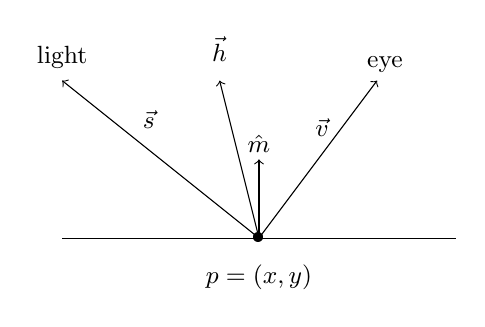
\begin{tikzpicture}
    \tikzstyle{every node}=[font=\small]
    % draw some lines
    \draw[black] (-1,0) -- (4,0);
    \draw[black, ->] (1.5,0) -- (-1,2);
    \draw[black, ->] (1.5,0) -- (3,2);
    \draw[black, ->] (1.5,0) -- (1.5,1);
    \draw[black, ->] (1.5,0) -- (1,2);
    % draw labels
    \node at (-1,2.3) {light};
    \node at (1,2.4) {$\vec{h}$};
    \node at (0.1,1.5) {$\vec{s}$};
    \node at (2.3,1.4) {$\vec{v}$};
    \node at (1.5,1.2) {$\hat{m}$};
    \node at (3.1,2.2) {eye};
    \node at (1.5,-0.5) {$p=(x,y)$};
    \node at (1.5,0) {\textbullet};
\end{tikzpicture}
\caption{Representation of our problem in two dimensions}
\label{fig:vectors}
\end{figure}

The vectors in the figure are defined as follows.
\begin{eqnarray*}
    s &=& light - p\\
    v &=& eye -p\\
    h &=& \frac{v+h}{2}
\end{eqnarray*}

As discussed in class we use use the formula in (\ref{eq:light_eq}) to
calculate color value (RGBA) for a given point. In this problem we
are only focusing on the color value without the alpha value.

\begin{equation}
    I = I_a P_a + I_d P_d \times lambert + I_s P_s \times Phong^f
    \label{eq:light_eq}
\end{equation}

Before we apply this formula let try to make sense of it and connect it
with our figure (\ref{fig:vectors}).

The first part of (\ref{eq:light_eq}) is the ambient light. No positions or
direction affect the ambient value. If some light affect some point this will
be added to the color value.

The second part of (\ref{eq:light_eq}) favors the diffuse light.
The diffuse part of the light is a function of the light-vector $s$ and the
direction of the normal $m$. This happens in the lambert part of the formula
where lambert is defines as follows.
\begin{equation*}
    lambert = max\left( \frac{s \cdot m}{|s||m|} \right) 
    \label{eq:lambert}
\end{equation*}

The third part of (\ref{eq:light_eq}) favors the specular light. Specular
lighting takes into account the position of the camera where we are calculating
reflection of light from the light source to the camera.  Like discussed in
class -- calculating this can be expensive. Therefore we use halfway vector $h$
as our reflection vector. This happens in the phong part of the formula where
phong is defined as follows,
\begin{equation*}
    phong = max\left( 0, \frac{h \cdot m}{|h||m|} \right)
    \label{eq:phong}
\end{equation*}
The power of phong in the formula is the specular shininess value.

Now we have defined everything we need to solve the problem so let us get busy.

We begin by calculate the vectors that we need, that is $s$, $v$ and $h$. We
calculate $s$ as follows.
\begin{eqnarray*}
    s &=& light - p\\
    &=& (-1,7,5) - (3,7,2)\\
    &=& (-4, 0,3)
\end{eqnarray*}


We calculate $v$ as follows.
\begin{eqnarray*}
    v &=& cam - p\\
    &=& (5,7,7) - (3,7,2)\\
    &=& (2, 0, 5)
\end{eqnarray*}

We calculate $h$ as follows.
\begin{eqnarray*}
    h &=& s+v\\
    &=& (-4,0,3) + (2,0,5)\\
    &=& (-2, 0, 8)
\end{eqnarray*}

Next we calculate Lambert and Phong. We calculate Lambert as follows.
\begin{eqnarray*}
    \textnormal{Lambert} &=& max\left( 0, \frac{s \cdot m}{|s||m|} \right)\\
    &=& max\left( 0, \frac{3}{5} \right)\\
    &=& \frac{3}{5}
\end{eqnarray*}

We calculate Phong as follows.
\begin{eqnarray*}
    \textnormal{Phong} &=& max\left( 0, \frac{h \cdot m}{|h||m|} \right)\\
    &=& max\left( 0, \frac{8}{\sqrt{68}} \right)\\
    &=& \frac{8}{\sqrt{68}}
\end{eqnarray*}

We can now calculate the blue color value for the point.
\begin{eqnarray*}
    I_B = (0 \times 0.2) + \left(0.2 \times 0.6 \times \frac{3}{5}\right) + \left(0.7 \times 0.9 \times \left(\frac{8}{\sqrt{68}}\right)^{13}\right)
\end{eqnarray*}

We then add the global ambience light to the value.
\begin{eqnarray*}
    I_B &=& I_B + \left[ 0.4 \times 0.2 \right]\\
    I_B &=& 0.57
\end{eqnarray*}

The blue value for the point, with this setting is $0.57$.


\pagebreak
\section*{Solution to problem 2}
Describe what happens when the following code is run and show the values that
will end up in the Projection matrix.
\begin{enumerate}
    \item gluPerspective(90, 1.25, 10,110);
\end{enumerate}

The function \texttt{gluPerspective(fovy, aspect, N, F);}\\calls the function
\texttt{glFrustrum(left,right, bottom, top, nearVal, farVal);}
where:
\begin{itemize}
    \item $top = N * tan\left( \frac{angle}{2} \right)$
    \item $bottom = -top$
    \item $right=top*ratio$
    \item $left=-bottom$
\end{itemize}
The function \texttt{glFrustrum} the multiples the current matrix, The projection matrix, with the following
matrix:
\begin{equation}
    \begin{bmatrix}
        \frac{2N}{right-left} & 0 & \frac{right+left}{right-left} & 0\\
        0 & \frac{2N}{top-bottom} & \frac{top+bottom}{top-bottom} & 0\\
        0 & 0 & -\frac{(F+N)}{F-N} & -\frac{2FN}{F-N}\\
        0 & 0 & -1 & 0
    \end{bmatrix}
\end{equation}
With all this we can fill into this matrix, where:
\begin{itemize}
    \item $top = N * tan\left( \frac{angle}{2} \right) = 10tan45^{\circ} \approx 10$
    \item $bottom = -top \approx = -10$
    \item $right=top*ratio = 10*1.25 = 12.5$
    \item $left=-bottom = -12.5$
\end{itemize}
The projection matrix becomes
\begin{equation}
    \begin{bmatrix}
        0.8 & 0 & 0 & 0\\
        0 & 1 & 0 & 0\\
        0 & 0 & -1.2 & -22\\
        0 & 0 & -1 & 0
    \end{bmatrix}
\end{equation}





\end{document}
